\documentclass[12pt]{article}
\usepackage{fontspec}
\setmainfont{Open Sans}
\usepackage{graphicx}
\usepackage{amsmath} 
\usepackage[utf8]{inputenc}
\usepackage{hyperref}

\hypersetup{
colorlinks=true,
    linkcolor=blue,
}
\graphicspath{ {./images/} }

\usepackage{listings}

\usepackage{titletoc,tocloft}
\setlength{\cftsubsecindent}{2cm}
\setlength{\cftsubsubsecindent}{4cm}
\setcounter{tocdepth}{2}
\dottedcontents{section}[1.5em]{}{1.3em}{.6em}
\usepackage[margin=1in]{geometry}

\author{Sammarth Kumar}
\title{Fluid Mechanics and Newton's Laws of Motion in Paper Airplanes}
\begin{document}
\maketitle
\tableofcontents
\newpage
\section{Abstract}
Paper planes can fly very far if built correctly. The world record for a paper plane is 226 feet 10 inches which is pretty far for a piece of paper. I wanted to see what different factors could affect a plane's flight and did so by modifying my plane based on four things: Thrust, lift,drag, weight. I designed and conducted my own experiment to see how these modifications would affect the speed, lift and orientation of the plane. The results align with known physics, thus making my experiment successful.
\section{Theory and Concepts Used}
\begin{figure}[h!]
\begin{center}
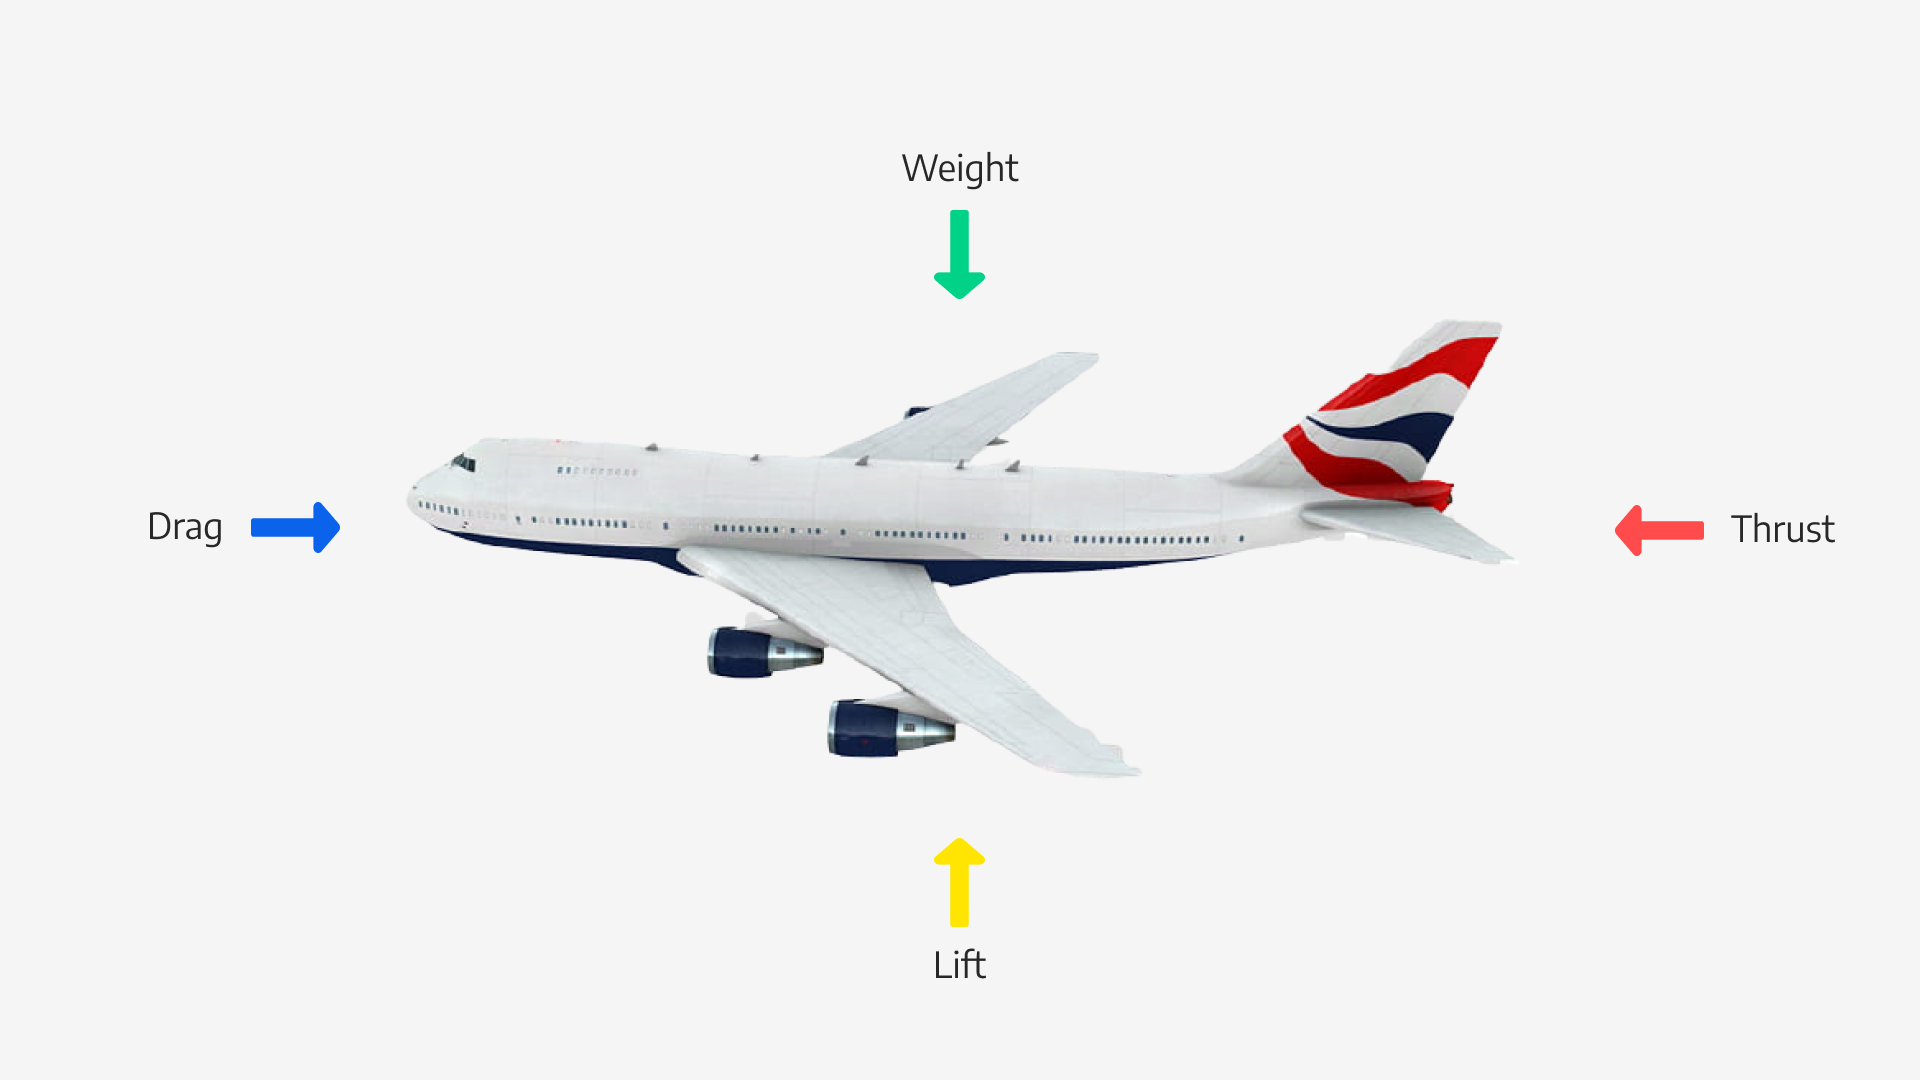
\includegraphics[scale=0.15]{plane1}
\end{center}
\caption{Forces acting on a plane}
\label{fig:Plane Diagram}
\end{figure}
As seen in \ref{fig:Plane Diagram}, there are four \emph{major} forces acting on the plane:
\begin{enumerate}
\item Thrust: force propelling it forward
\item Lift: force pushing it upward
\item Weight: force pulling it down
\item Drag: force opposing motion
\end{enumerate}
Planes fly because of the various ways they are engineered to make the most efficient and practical use of each force for the required purpose.
At the same time, commercial planes and military jets are designed differently, the former with the most fuel efficient design and the second with a design to achieve great speeds. That's why fighter jets are smaller, more compact and also have features which commercial planes do not. On the other hand, charter planes are much bigger with a much larger wingspan and are designed to fly at a good speed while maximising fuel efficiency.

\subsection{Thrust}
When we talk about thrust, in the case of real planes, engines provide the necessary thrust to propel the plane. In a paper airplane, we generate thrust by throwing the plane.

\subsection{Lift (Bernoulli's Principle, Coandă Effect, Third Law of Motion)}
\begin{figure}[h!]
\begin{center}
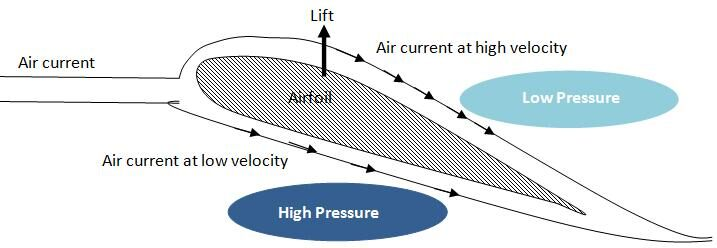
\includegraphics[scale=0.4]{dynamic}
\end{center}
\caption{Dynamic Lift from Bernoulli's Principle}
\label{fig:Dynamic Lift}
\end{figure}
Lift has been a topic of great controversy. It was originally thought that it could be explained through \emph{Bernoulli's Principle} since it was assumed that air on top of a wingfoil had to cover a greater distance and hence had a greater velocity resulting in a lower pressure area over the plane and causing an upward force as air tried to regain equilibrium. This assumption was proved wrong in an experiment which showed that the upper and lower layers never meet and the upper layer actually reaches the end before the lower one.

Another explanation is based off the Coandă Efect and Newton's Third Law as seen in \ref{fig:Coandă Effect}. As per the Coandă Effect, the particles of a fluid stick to a body moving through it and similarly, they stick to the curve of a wing. As the top layer of air moves downwards, the bottom layer is also forced in the same direction and they exert an equal and opposite force on the wing as per \emph{Newton's Third Law}. This and some other factors produce lift.
\newpage
\begin{figure}[h]
\begin{center}
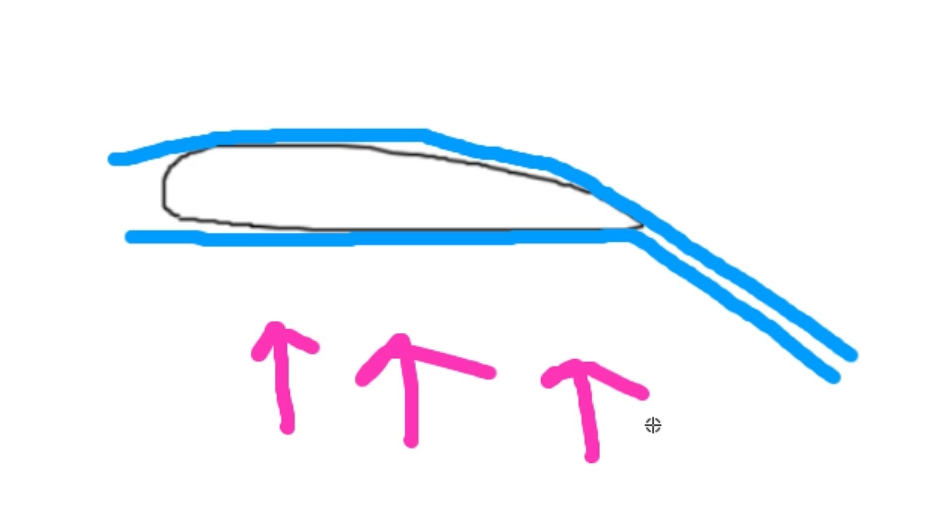
\includegraphics[scale=0.4]{wing}
\end{center}
\caption{Coandă Effect and Newton's Third Law}
\label{fig:Coandă Effect}
\end{figure}
Different sources have different explanations, but the second seems more plausible since the \emph{Equal Time Argument} has its flaws. From either theory, the general consensus is that lift is directly proportional to the relative velocity and surface area of the wing, which is really what this experiment is about.
\subsection{Weight and Second Law of Motion}
The weight is the action of the gravitational force exerted on the plane by the earth. Its magnitude is given by the formula (from \emph{Newton's Second Law of Motion}):
\begin{equation}\label{eq:weight}
F = mg
\end{equation}
Where \emph{g} is acceleration due to gravity.
\subsection{Center of Mass}
Center of mass is the hypothetical point where all the weight is balanced and was created to simplify calculations. It is assumed that forces act on this point, including but not limited to \emph{gravitational force}.

\subsection{Drag}
Drag is a force that opposes the motion of the plane. In this project we deal with mainly pressure drag and viscous drag, although other kinds do exist.

To calculate force exerted due to pressure drag, we can make use of \emph{the Modern Drag Equation} (derived from Bernoulli's equation) which gives the following relation:

\begin{equation}\label{eq:drag equation}
R = \frac{1}{2} \rho C A v^{2} 
\end{equation}

This gives us:
\begin{equation}
R \propto v^{2}
\end{equation}
\begin{equation} 
R \propto A
\end{equation}
Here, $C$ is called the coefficient of drag and is measured experimentally and accounts for other factors (body shape, inclination, air viscosity, and compressibility, etc.). $\rho$ is the density of air, \emph{A} is the reference area and \emph{v} is the velocity.

That's why planes are streamlined and why fighter jets and planes like Concord are as compact as possible - to reduce surface area and minimise drag, which allows them to achieve great speeds.
\subsection{Terminal Velocity and Stoke's Law}
Terminal velocity is the maximum velocity attainable by an object as it falls through a fluid. It is proportional to the force exerted by a body moving through a fluid, as per \emph{Stoke's Law}.

In our paper plane, there are some other factors which affect the velocity of the plane as well, but
the concept of Terminal Velocity can be used to explain some of the phenomena seen.
\begin{equation}\label{eq:Stoke's Law}
F \propto v
\end{equation}
\section{Procedure}
To conduct the experiments, I modified certain features of the standard paper airplane:
\begin{enumerate}
\item Thrust Given
\item Surface Area
\item Wingspan
\item Center of mass
\end{enumerate}

The experiment can be seen in \href{https://youtu.be/qcbdRIKSDts}{this video}. I conducted this in an enclosed room to avoid external forces and create as controlled an environment as possible. The only limitation was that the room was small so the plane ended up hitting a surface. However, there was enough distance to see the effect of the changes I made to the plane.
\section{Results}
From the experiments conducted in \href{https://youtu.be/qcbdRIKSDts}{this video}, I got the following results:
\begin{figure}[h!]
\begin{center}
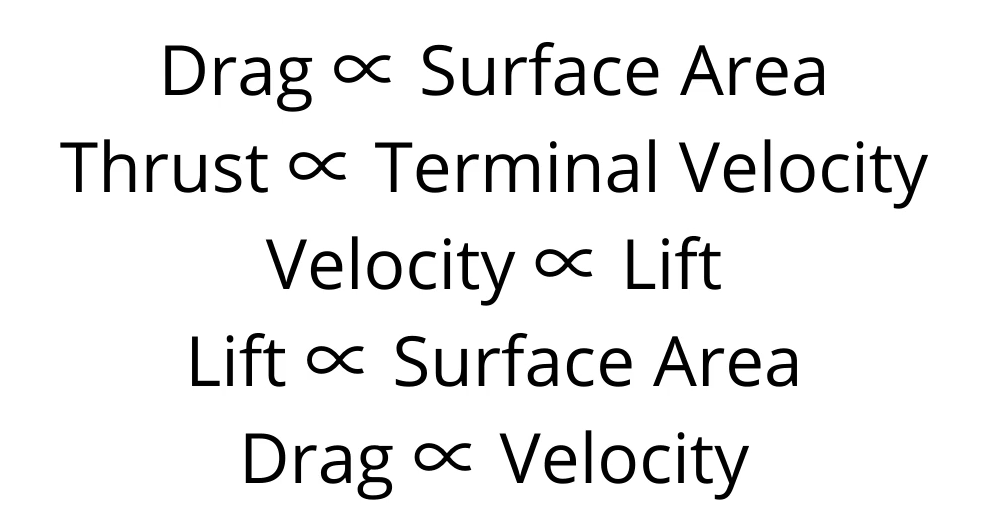
\includegraphics[scale=0.4]{conclusions}
\end{center}
\caption{Results}
\label{fig:results}
\end{figure}
\paragraph{}
As seen in \ref{fig:results}, our observations align with previously determined relations between the given physical quantities
\section{Conclusion}
\subsection{Summary}
In conclusion, the experiment verified previously deduced results and also gave an insight into how different factors affect the flight of a plane.
\subsection{What I Learned}
In this project, I learned a lot about how planes fly and how they are engineered to perfection to maximise efficiency and purpose. I learned how to design my own experiment to test different phenomenon and how to present my findings in a scientific method.
\section{Bibliography}
\begin{enumerate}
\item ThePaperAirplaneGuy (\url{https://www.youtube.com/user/ThePaperAirplaneGuy})
\item Learn Engineering (\url{https://www.youtube.com/user/LearnEngineeringTeam})
\item Cambridge University (\url{https://www.cam.ac.uk/research/news/how-wings-really-work})
\item NASA (\url{https://nasa.gov})
\item Doofer911 (\url{https://www.youtube.com/watch?v=YDeQXPNpLeY})
\end{enumerate}
\end{document}
